%% Match the Router to the Regime: Shadow-Price Two-Tier Routing for Pipelined VLM Inference on the LEO Satellite Edge
%% INFOCOM format. Compile with pdfLaTeX + BibTeX.
\ifdefined\pdfminorversion\pdfminorversion=7\fi  % allow the v1.7 PDF figure (pdfLaTeX only)
\documentclass[10pt, conference, letterpaper]{IEEEtran}
\IEEEoverridecommandlockouts

\usepackage{url}
\usepackage{graphicx}
\usepackage{subfigure}
\usepackage{booktabs}
\usepackage{array}
\usepackage{amsmath,amsthm,amssymb,amsfonts,autobreak}
\usepackage{pifont}
\usepackage[ruled,vlined,linesnumbered]{algorithm2e}
\usepackage[table,xcdraw]{xcolor}
\usepackage{colortbl}
\usepackage{bm,epsfig,amsthm,url}
\usepackage{verbatim}
\usepackage{cite}
\usepackage{tabularx}
\usepackage{mathrsfs}
\usepackage{tikz}
\usetikzlibrary{arrows.meta,positioning}
\graphicspath{{figs/}}
\hyphenation{op-tical net-works semi-conduc-tor}
\SetCommentSty{\textit\footnotesize} 

\begin{document}

\title{ELARA: Efficient Microservice Orchestration for Latency and Energy in Space Computing Power Networks
}
% \title{Microservices Routing in Space Computing Power Networks}

\author{\IEEEauthorblockN{Anonymous Authors}}

\maketitle 

\begin{abstract}
Recent advances in the communication and computing capabilities of low Earth orbit satellites enable their key role in space computing power networks (SCPNs) and in-orbit intelligent service provision. Constrained by limited onboard resources, deploying these complex, monolithic applications on a single satellite is practically infeasible. Microservice architecture provides a promising solution by decomposing applications for distributed execution across the constellation. Nevertheless, orchestrating these microservices is nontrivial due to time-varying, heterogeneous SCPN environments and the tight coupling between serving-satellite selection, data routing, and service replica placement.
To this end, we present ELARA, an online microservice orchestration framework that coordinates serving satellite selection, routing across slots, and service replica adaptation under dynamic SCPN environments. Specifically, ELARA first employs a graph neural network-enhanced proximal policy optimization agent for serving satellite selection by capturing the communication and computation states. Then, it adopts a time-slot-aware min-cost max-flow routing module with residual data updates to support parallel and cross-slot service data transmission. On this basis, ELARA designs a bandit-based replica adaptation strategy to relocate hotspot service replicas at the orbital-plane level with low decision overhead. Extensive simulations under dynamic LEO constellation topologies demonstrate that ELARA achieves lower end-to-end latency and mean execution energy than representative baselines.


\end{abstract}

\section{Introduction}
\label{sec:intro}
 In recent years, large-scale LEO satellite networks have garnered widespread attention as one of the recognized highlights of 6G technology~\cite{shi2025satellite}.
 Modern LEO mega-constellations, consisting of hundreds to thousands of LEO satellites connected by inter-satellite links (ISLs), enable the globally ubiquitous connections~\cite{net_char_StarLink_LEO}.
 Meanwhile, advancements in remote sensing and chip technology have enabled modern LEO satellites to be equipped with high-performance imaging and intelligent computing payloads~\cite{mi2019intelligent, shen2023survey}, thus supporting ubiquitous intelligent services such as weather forecasting, environmental monitoring, and national security~\cite{satellite_sys_survey, progress_challenge_RS_satellite}.
 Hundreds to thousands of satellite computing nodes collectively form the SCPNs, as show in Fig.~\ref{fig:sys_scenario}, where the strategic service routing and deployment to efficiently fulfill diverse intelligent service requests has emerged as a critical challenge in the context of 6G integrated space-air-ground networks~\cite{SAG_survey_6g}.


%Recent advances in low Earth orbit (LEO) mega-constellations are transforming satellites from communication relays into distributed computing nodes in space.
%These constellations, consisting of hundreds to thousands of satellites connected by inter-satellite links (ISL) and equipped with onboard processors and storage, enable global connectivity and near-data processing~\cite{net_char_StarLink_LEO,satellite_sys_survey}.
%This evolution is particularly critical for Earth observation, weather forecasting, environmental monitoring, and remote sensing analytics, where massive volumes of images and multimodal data are continuously generated in orbit~\cite{shi2025satellite,progress_challenge_RS_satellite,seco_infocom2024}.
%As shown in the left half of Fig.~\ref{fig:sys_scenario}, directly downloading such raw data to terrestrial data centers consumes scarce ground-to-satellite link bandwidth and worsens link congestion, hindered by limited visibility windows and unstable channel conditions~\cite{leyva2023satellite,joint_orbit_comp_comm4data_Download}.
%Consequently, space computing power networks (SCPNs), as illustrated in Fig.~\ref{fig:sys_scenario}, integrate sensing, communication, and computing resources across LEO satellites, making them a promising infrastructure for onboard intelligent services~\cite{shi2025satellite,survey_on_nextg_comp_tech_SAGIN}.

Despite this promise, running complex monolithic applications on a single LEO satellite remains infeasible because each satellite has limited computing, storage, energy, and thermal dissipation capabilities~\cite{leyva2023satellite,joint_orbit_comp_comm4data_Download}.
Microservice architecture provides an effective solution by decomposing these monolithic applications into small, loosely coupled, and reusable microservices, each encapsulating a distinct functional module~\cite{3D_assets_microservice}.
By packaging them into lightweight containers and deploying them across interconnected satellites, as shown in Fig.~\ref{fig:sys_scenario}, this architecture alleviates individual satellite resource limitations and enables onboard cooperative execution.
%Hotspot microservices can also be dynamically scaled or redeployed to support robust service provisioning.

Typically, we consider a request initiated by a terrestrial user that consists of a subset of microservices. During the execution, the dynamic constellation topology can slow down or even interrupt this process because of time-varying and intermittent inter-plane ISLs.  Moreover, hardware heterogeneity and limited onboard energy further complicate scheduling decisions at each microservice execution stage.


In this contxt, enabling energy-efficient and low-latency service provisioning in SCPNs requires addressing three major challenges.
First, the satellite network topology is predictable but varies rapidly over time. As illustrated in Fig.~\ref{fig:time_varying_isl}, intra-plane ISLs are relatively stable, whereas inter-plane ISLs are sensitive to satellite motion and vary frequently across slots. Consequently, data transmission over ISLs can suffer from link disruptions, congestion, or degraded transmission rates.
Second, serving satellite selection and data routing are tightly coupled. Selecting a nearby satellite that hosts called service replica may reduce transmission delay but suffer long computation queues, whereas an idle satellite may incur high communication cost over many hops~\cite{energy_efficient_routing_tsinghua,cao_comp_routing}. 
%This tradeoff is further complicated by heterogeneous computing capacities and energy constraints~\cite{energy_efficient_routing_tsinghua,cao_comp_routing}.
Third, microservice replica deployment across satellites cannot remain static~\cite{yu_deploy_tmc2025}. As user requests, satellite workloads, and constellation topology evolve, previously effective placements can become inefficient. 
A practical controller must identify the bottleneck services and adapt their placement periodically for latency reduction and energy saving.

Existing studies have extensively investigated satellite edge computing, computation offloading, service deployment, and data routing over ISLs in SCPNs~\cite{leyva2023satellite,joint_orbit_comp_comm4data_Download,sc_nfv_tmc2024,service_pressure,yu_deploy_tmc2025}.
Nevertheless, most existing solutions do not coordinate request execution and service deployment to adapt to changing communication conditions and onboard computation workloads.
In particular, existing service and function execution models for satellite networks commonly assume that each task is completed within a single time slot under a fixed constellation snapshot, while treating service routing and deployment as separate problems.
Although these assumptions simplify modeling and algorithm design, they do not capture practical service execution in orbit, where data routing and computation may span multiple time slots and deployment decisions directly affect subsequent request execution~\cite{cross_slot_optim_infocom2025}.
Terrestrial microservice studies have jointly considered service deployment and request routing~\cite{optim_svc_dep_req_reouting_in_MEC}, but their assumptions of stable networks, abundant power, and fixed edge infrastructure do not directly apply to SCPNs.

\begin{figure}[!t]
\centering

\includegraphics[width=1\linewidth]{figs/sys_scenario.pdf}
\vspace{-0.5cm}
\caption{SCPN scenario for microservice provisioning in orbit.}
\label{fig:sys_scenario}
\vspace{-0.7cm}
\end{figure}

\subsection{Contributions}
To address these challenges, we propose ELARA, an energy-efficient and latency-aware  microservice orchestration framework for SCPNs. ELARA coordinates serving satellite selection, routing across slots, and replica adaptation under one objective over the decision horizon using two decision timescales. For each request, the fast control loop selects a serving satellite for every microservice stage and reserves transmission capacity over the current ISL topology. Over a longer deployment window, the slow control loop ranks services by their contribution and adjustment potential. It then decides whether each of up to $K_{\mathrm m}$ services with the highest pressure should retain its deployment or relocate one replica under the onboard memory constraint.

In summary, the main contributions are as follows:
\begin{enumerate}
\item
We formulate online microservice orchestration in a dynamic SCPN under one objective over the decision horizon that accounts for request latency and communication and computation energy. The formulation exposes the different decision rates of request execution and replica adaptation and motivates a solution with two decision timescales.

\item
We design a fast control loop that combines serving satellite selection using a graph representation with routing over ISLs whose states vary over time. The routing procedure reserves capacity only for data that can reach the selected serving satellite within the current slot. Undelivered data remains at the source satellite and is routed again after the topology update, which leaves no ambiguity about its location.

\item
We design a slow control loop that measures service pressure from request outcomes and applies one contextual bandit decision to each of up to $K_{\mathrm m}$ services with the highest pressure. Each decision either retains the current deployment or relocates the replica with the largest observed service cost to a satellite in another orbital plane that has sufficient memory. A shared linear model learns from the subsequent change in service cost, and a retention action prevents unnecessary deployment changes.

\item
We evaluate ELARA using dynamic LEO topology traces and microservice workloads. The results show lower request latency and execution energy than representative satellite computing and service routing baselines and quantify the contributions of serving satellite selection, routing across slots, and replica adaptation.

\end{enumerate}


%The remainder of this paper reviews related work, presents the system model and problem formulation, details ELARA, evaluates its performance, and concludes the paper.
The remainder of this paper is organized as follows.
Sec.~\ref{sec:related_work} reviews the related work.
Sec.~\ref{sec:sys_model} presents the system model.
The problem formulation is introduced in Sec.~\ref{sec:prob_form}.
Sec.~\ref{sec:algo} details the proposed ELARA framework.
Sec.~\ref{sec:eval} presents the performance evaluation.
Sec.~\ref{sec:conclusion} concludes the paper.

\begin{figure}[!t]
\centering
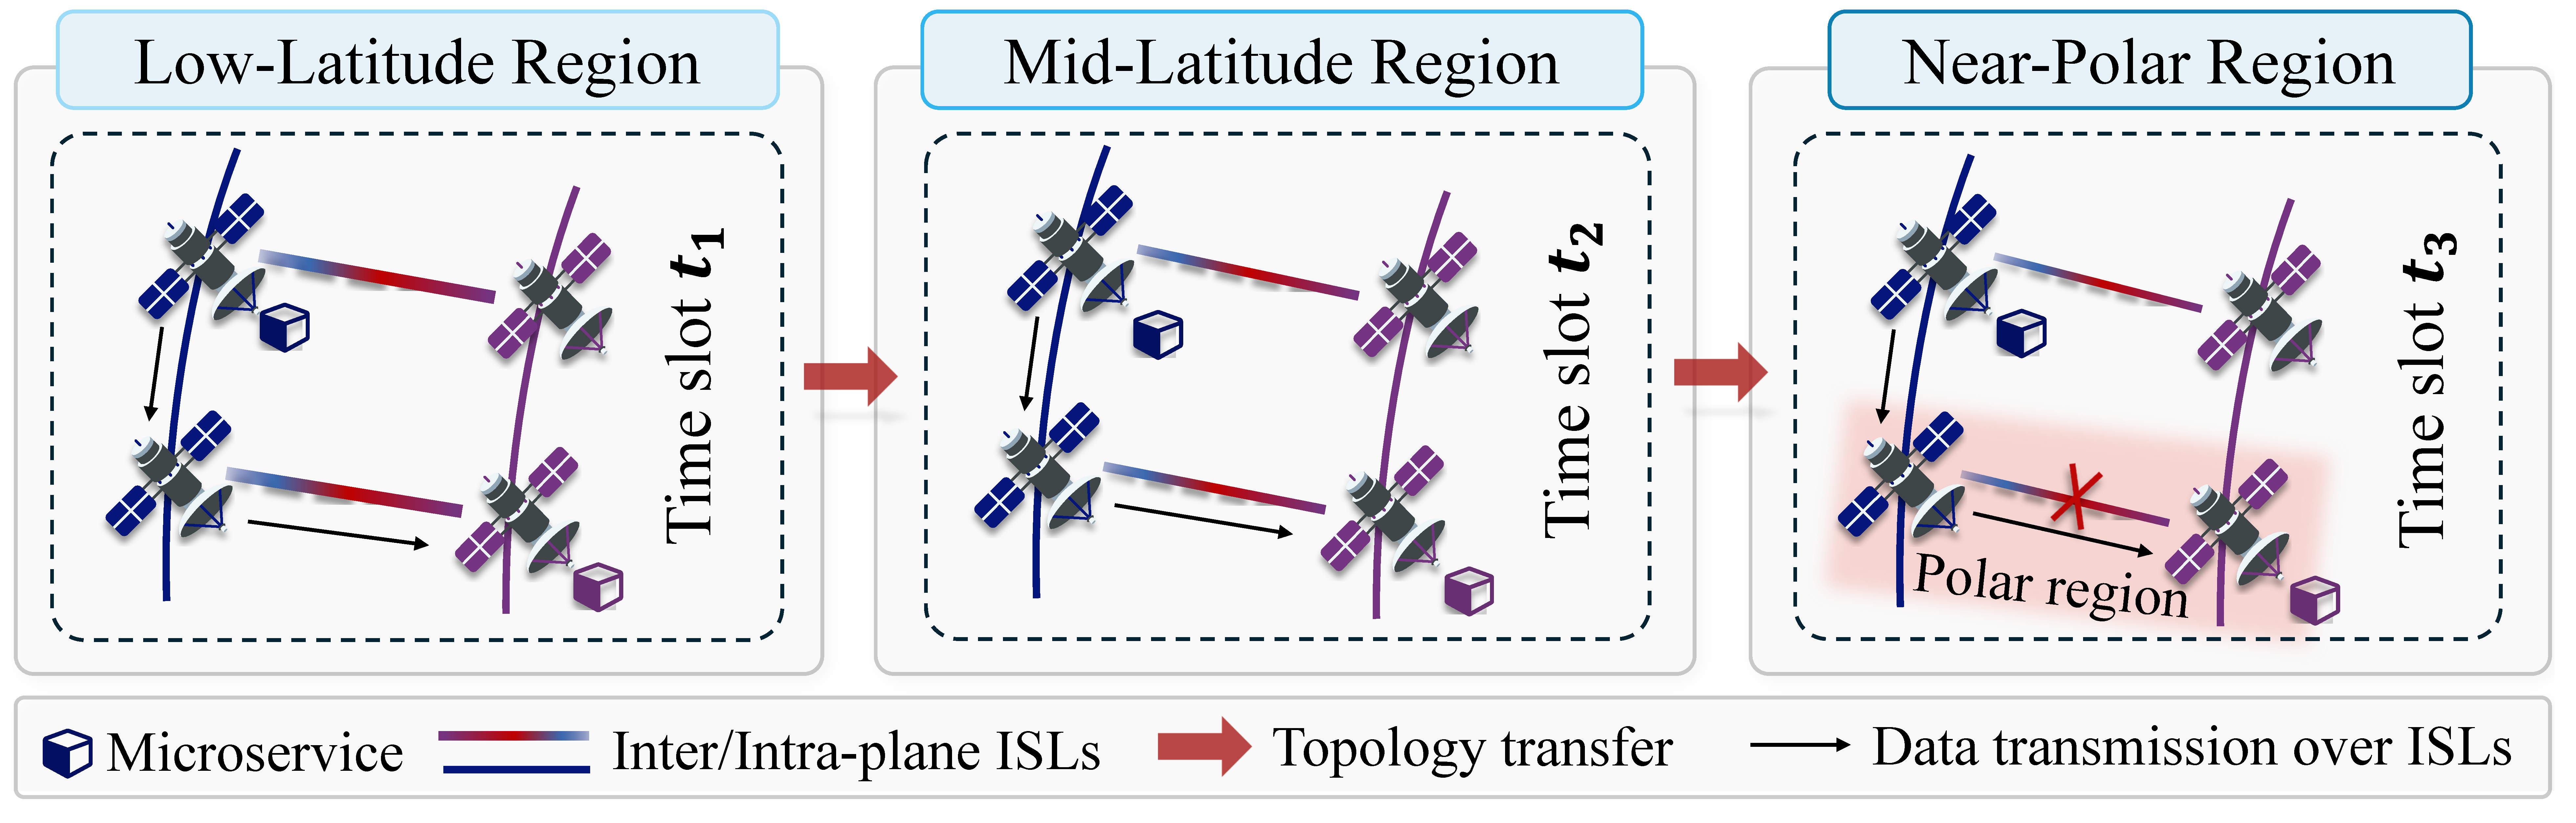
\includegraphics[width=1\linewidth]{figs/time_varying_isl.pdf}
\vspace{-0.6cm}
\caption{LEO topology with dynamic ISLs between orbital planes.}
\label{fig:time_varying_isl}
\vspace{-0.7cm}
\end{figure}

\section{Related Work}
\label{sec:related_work}

% Recent advancements in satellite edge computing and SCPNs have supported near-data processing over LEO constellations with onboard computation and ISL connectivity \cite{survey_on_nextg_comp_tech_SAGIN,SAG_integ_net,xie2020stec,sate_computing_case_study}.
% Zhang et al. \cite{zhang2023sec_offloading} investigated energy-efficient peer offloading among satellites, where computation tasks are cooperatively migrated to reduce energy consumption.
% Leyva-Mayorga et al. \cite{leyva2023satellite} studied satellite edge computing for real-time very-high-resolution Earth observation, and Zhai et al. \cite{seco_infocom2024} proposed SECO to jointly optimize multi-satellite observation scheduling, routing, and computation node selection.
% These efforts mainly focus on task-level offloading, mission-specific processing, or computation-communication resource allocation.
% Microservice-oriented service provision, however, introduces finer-grained execution dependencies across distributed replicas, where intermediate data transmission and onboard computation are tightly coupled under dynamic SCPNs.

Recent advances in satellite edge computing and SCPNs have enabled data processing directly in LEO constellations with onboard computation and ISL connectivity~\cite{shi2025satellite,survey_on_nextg_comp_tech_SAGIN,xie2020stec}.
Zhang et al.~\cite{zhang2023sec_offloading} investigated energy efficient peer offloading among satellites, while Leyva-Mayorga et al.~\cite{leyva2023satellite} and Zhai et al.~\cite{seco_infocom2024} explored Earth observation with strict timing requirements and joint optimization of observation scheduling, routing, and computation node selection.
These studies primarily focus on task offloading, processing for a specific mission, or joint allocation of computation and communication resources, whereas microservice provisioning introduces execution dependencies among distributed replicas at a finer granularity.

% Service routing and task scheduling in satellite networks have also been studied from various of perspectives.
% In \cite{cao_comp_routing}, the author proposed a computing-aware routing framework that integrates transmission and computation decisions for remote sensing tasks in LEO satellite networks.
% Xia et al. \cite{sc_nfv_tmc2024} studied service chaining in NFV-enabled satellite edge networks, while Abreha et al. \cite{fairness_vnf_tnsm2024} considered fairness-aware VNF mapping and scheduling for mission-critical services.
% For improve routing effiency and avoiding link congestion, He et al. \cite{service_pressure} investigated throughput-oriented routing for microservice flows in LEO satellite networks.
% Moreover, some works further model dynamic networks with time-expanded graphs or optimize routing over time-varying LEO topologies \cite{liu2023time_expanded_graph,routing_optim_in_multi_domain,cross_slot_optim_infocom2025}.
% However, most of them either optimize communication paths alone or consider computation-node selection within a given stable topology snapshot or a pre-defined topology sequence.
% They fails to capture the joint impact of broken inter-plane ISLs, heterogeneous serving node computing capacity, and time-varying SCPNs for microservice requests.

Service routing and task scheduling in satellite networks have also been studied from multiple perspectives.
Cao et al.~\cite{cao_comp_routing} proposed routing that considers computing states for remote sensing tasks, Xia et al.~\cite{sc_nfv_tmc2024} investigated service chaining with network function virtualization, and He et al.~\cite{service_pressure} developed routing for microservice flow throughput. Other studies model dynamic topologies using graphs expanded over time or optimize routing over LEO constellations that vary over time~\cite{liu2023time_expanded_graph,routing_optim_in_multi_domain,cross_slot_optim_infocom2025}.
However, most of these works either focus on communication paths alone or consider computation node selection within static topology snapshots or predefined sequences, leaving the joint impact of ISL disruptions, heterogeneous computing capacities, and topology variation insufficiently addressed.


Microservice deployment and request execution have been extensively studied in terrestrial edge systems.
Peng et al.~\cite{optim_svc_dep_req_reouting_in_MEC} studied joint service deployment and request routing in mobile edge computing. In satellite environments, Gao et al.~\cite{optim4server_svc_place_in_STIECN} investigated joint server and service selection, and Yu et al.~\cite{yu_deploy_tmc2025} developed robust reinforcement learning for microservice deployment in SCPNs.
Nevertheless, existing methods are either designed for static terrestrial scenarios or induce prohibitively large decision spaces when satellite selection and service deployment are considered together. Coordinating request execution with replica deployment under dynamic computing conditions and changing ISLs therefore remains an open challenge.


\begin{comment}
\section{Related Work}
\label{sec:related_work}
%\subsection{Satellite (space) edge computing (energy-aware)}
Recent advancements in satellite technology have significantly promoted its computing and transmitting capabilities, enabling satellites to undertake some elementary tasks \cite{survey_on_nextg_comp_tech_SAGIN}.
The construction of ISLs, in particular, enables interconnected satellites to form the SCPN with pooled computing resources, supporting intricate missions with enhanced performance demands \cite{space_asisit_comp_offload4IoTApp,leyva2023satellite, sate_computing_case_study}
and facilitating a global response to requests from anywhere at any time\cite{IPIS_sate, laser_sate}.
In addition,
% due to the poor power system of satellites,
careful energy management is necessary for satellites to realize sustainable development \cite{energy_efficient_routing_tsinghua, energy_drain_attact_on_satellite}.

Considering the discrete distributed computing nodes (as satellites) with limited computing power in the SCPN, researchers have migrated the monolithic applications (such as 3D reconstruction and inference model), which are traditionally deployed on ground data centers, to space networks by decomposing them into microservices, which are characterized by being independent, scalable, reusable, and stateless\cite{geoAIasMicroService,3D_assets_microservice,ye2024galaxy}.
These microservices can be scaled and deployed on the satellites through platform-independent containerization technology, which encapsulates these isolated microservices into containers that are transparent to the installed computing platform on satellites \cite{Docker,SAG_integ_net}.

Extensive research has been conducted on service routing algorithms, aiming at the problems of node selection and routine planning.
Fu et al. \cite{energy_alloc_addmission_ctrl4comm_satellite} proposed a dynamic programming approach to drive the optimal policy on energy allocation for a single satellite in response to user requests. It fails to consider the multi-satellite cases.
The work \cite{optim4server_svc_place_in_STIECN} designed a joint edge server placement and service deployment model for SAGIN, aiming to minimize the average response latency and energy cost.
The work \cite{energy_efficient_routing_tsinghua} developed a series of heuristic algorithms to prolong the serving life of satellites by switching part of routers installed on satellites to sleep mode, and resolving the energy-efficient routing policies.
Efficient but shortsighted, these proposed algorithms cannot adapt to diverse routing needs, for example, the treed topology raised by requested missions, which demands integrated computing and communication routing as well as multi-satellite collaboration.
\end{comment}


\section{System Model}
\label{sec:sys_model}

We consider an SCPN built upon a classic Walker Delta LEO constellation, where satellites are connected through laser ISLs and equipped with constrained onboard computing and storage resources.
Microservice applications are deployed as stateless replicas across satellites, allowing each request to be collaboratively executed through successive communication and computation stages.

% We consider a space computing power network (SCPN) composed of a Walker-Delta LEO constellation, where each satellite is equipped with onboard computing resources and laser inter-satellite links (ISLs).
% User tasks are represented as ordered microservice chains.
% Each microservice can have multiple stateless replicas deployed on different satellites, and a request may therefore be executed collaboratively by multiple satellites.
% The key distinction from terrestrial edge systems is that the SCPN simultaneously exhibits predictable but fast topology dynamics, intermittent inter-plane ISLs, limited onboard compute and storage resources, and time-varying communication conditions.

\subsection{LEO Constellation and Topology Model}
\label{subsec:constellation_model_new}

A typical Walker Delta constellation is parameterized by $\mathcal{W}=(N_{\text{sat}}/P/G,h_{\text{orb}},I)$, where $N_{\text{sat}}$ is the total number of satellites, $P$ is the number of orbital planes, $G$ is the phasing factor between planes, $h_{\text{orb}}$ is the orbital altitude, and $I$ is the inclination.
Consequently, each orbital plane accommodates $N = N_{\text{sat}}/P$ satellites.
% A satellite node is uniquely identified by its orbital plane index $p$ and its intra-plane position index $n$, denoted by $v_{p,n}$.
The set of satellite nodes in the constellation is formally defined as $\mathcal{V}=\{v_{p,n}\mid p=1,\ldots,P,\ n=1,\ldots,N\}$, where $p$ denotes the orbital plane index and $n$ denotes the position index within that plane.
To capture the high dynamism of the satellite network, we discretize the constellation period into a set of time slots $\mathcal{T} = \{0, 1, \ldots, T-1\}$ with a uniform slot duration $\Delta$.
For any instant $\tau$ in continuous time, the corresponding slot index is $s(\tau) = \left\lfloor \tau/\Delta \right\rfloor \bmod T$.
Using graph snapshots, we assume that the network state, including satellite positions, ISL availability, and capacity, remains unchanged within a slot and evolves only at slot boundaries, as shown in Fig.~\ref{fig:time_varying_isl}.
Thus, the network topology during slot $t \in \mathcal{T}$ is defined as a dynamic graph $\mathcal{G}(t) = \big(\mathcal{V}, \mathcal{E}(t)\big)$, where $\mathcal{E}(t)$ represents the set of feasible ISLs at slot $t$.
% Geometrically, the position of $v_{p,n}$ at slot $t$ is defined in spherical coordinates as $(H+R_E, \mho_p, \nu_{p,n}(t))$, where $R_E$ is the Earth's radius, $\mho_p$ is the $p$-th plane's right ascension of the ascending node (RAAN), and $\nu_{p,n}(t)$ is its orbital phase.

\subsection{ISL Communication Model}
We assume that each satellite is equipped with four laser optical terminals: two positioned along the roll axis for ISLs within its plane, and two along the pitch axis for ISLs between planes.

\paragraph{ISL Connectivity Constraints}
Each satellite $v_{p,n}$ maintains two ISLs with its adjacent neighbors $v_{p,n^-}$ and $v_{p,n^+}$ in the same plane, where $n^{\pm} = ((n \pm 1) \bmod N) + 1$.
Because satellites in the same plane share identical angular velocities, their relative distances remain constant over time, yielding highly stable communication links.

Conversely, ISLs between planes are dynamic.
Constrained by the physical limits of onboard laser communication terminals, the existence of a link $e=(u,v)$ between planes at slot $t$ is jointly determined by line of sight (LoS) distance, mechanical tracking thresholds, and polar exclusions, formulated as:
\begin{equation}
e\in \mathcal{E}(t) \iff \left\{
\begin{array}{l}
d_{u,v}(t) \le d_{\text{max}}, \\
\theta_{u,v}(t) \le \theta_{\text{max}}, \\
\max\big(|\varphi_u(t)|, |\varphi_v(t)|\big) \le \varphi_{\text{max}}.
\end{array}
\right.
\label{eq:cross_link_indicator}
\end{equation}
where the LoS distance $d_{u,v}(t)$ and relative tracking angle $\theta_{u,v}(t)$ are bounded by the terrestrial occlusion limit $d_{\text{max}}$ and the hardware threshold $\theta_{\text{max}}$, respectively.
Furthermore, the third constraint enforces a polar exclusion zone at latitude boundary $\varphi_{\text{max}}$ (e.g., $70^{\circ}$) by proactively tearing down links between planes, thereby avoiding the severe pointing dynamics and extreme Doppler shifts inherent to polar regions.
% This mechanism proactively tears down inter-plane links at high latitudes to bypass the severe pointing dynamics and extreme Doppler shifts inherent to polar regions.


\paragraph{ISL Capacity Model}
Unlike terrestrial networks with stable capacities, the transmission rate of laser ISLs depends on distance because of geometric propagation loss.
% Under the Free-Space Optical (FSO) communication model, the received optical power $P_{e}^{\text{rx}}(t)$ at satellite $v$ transmitted from satellite $u$ is formalized by the Friis transmission equation variant:
Based on the free space optical (FSO) communication model, the received power $P_{e}^{\text{rx}}(t)$ at satellite $v$ transmitted from satellite $u$ is formalized as:
\begin{equation}
P_{e}^{\text{rx}}(t) = P^{\text{tx}} G^{\text{tx}} G^{\text{rx}} \eta_{\text{tx}} \eta_{\text{rx}} \left(\frac{\lambda}{4\pi d_{u,v}(t)}\right)^2,
\label{eq:received_power}
\end{equation}
where $P^{\text{tx}}$ is the laser transmit power, $G^{\text{tx}}$ and $G^{\text{rx}}$ represent the optical gains of the transmitter and receiver apertures, respectively, $\lambda$ is the laser wavelength, and $\eta_{\text{tx}}, \eta_{\text{rx}}$ denote the optical efficiency factors.
The signal to noise ratio (SNR) of link $e$ at slot $t$ is given as:
\begin{equation}
\gamma_{e}(t) = \frac{\left({R}_{\text{pd}} \cdot P_{e}^{\text{rx}}(t)\right)^2}{\sigma_{\text{sh}}^2 + \sigma_{\text{th}}^2},
\label{eq:snr_formal}
\end{equation}
where ${R}_{\text{pd}}$ is the photodiode responsivity, while $\sigma_{\text{sh}}^2$ and $\sigma_{\text{th}}^2$ denote the shot and thermal noise variances, respectively.
% According to the Shannon-Hartley theorem, the achievable transmission capacity $R_{e}(t)$ (in bits per second) is constrained by:
According to the Shannon-Hartley theorem~\cite{IPIS_sate}, the achievable transmission capacity $R^0_{e}(t)$ is constrained by:
\begin{equation}
R^0_{e}(t) =  \text{B}_{e} \log_2 \left( 1 + \gamma_{e}(t) \right),
\label{eq:shannon_capacity}
\end{equation}
where $\text{B}_{e}$ is the modulation bandwidth.

\paragraph{ISL Delay Model}
The ideal rate $R^0_e(t)$ in \eqref{eq:shannon_capacity} could be degraded in practice by transient channel fading and traffic contention.
To capture these factors, we introduce a scaling factor $\eta_e(t)\in(0,1]$ to formulate the effective data rate as $R_e(t)=\eta_e(t)R^0_e(t)$.
When transmitting a data block of size $B$ over link $e=(u,v)$ during slot $t$, the aggregate communication delay comprises queuing, transmission, and propagation delays, formulated as:
\begin{equation}
T_e^{\text{cm}}(B,t) = \nu_e^{\text{qe}}(t) + \nu_e^{\text{tr}}(t) + \nu_e^{\text{pr}}(t).
\label{eq:link_delay_elara}
\end{equation}
Here, $\nu_e^{\text{qe}}(t)$ denotes the queuing delay, which can be dynamically estimated by probing queue lengths.
The transmission delay is given by $\nu_e^{\text{tr}}(t) = B / R_e(t)$, and the propagation delay is $\nu_e^{\text{pr}}(t)=d_e(t)/c$, with $c$ being the speed of light in vacuum.
% Crucially, this abstraction enables ELARA to implicitly account for network congestion without incurring the prohibitive overhead of tracking individual background flows.

% This compact model allows ELARA to account for link contention without explicitly modeling every concurrent background flow.

\subsection{Onboard Computing Model}
\label{subsec:compute_model_elara}

Let $F^0_v$ denote the ideal computing capacity of satellite $v$.
In practice, the available computational resources are often constrained by background payload tasks, operating system overhead, and thermal throttling~\cite{joint_orbit_comp_comm4data_Download}.
To capture these hardware and software limitations, we introduce a computational efficiency factor $\xi_v(t)\in(0,1]$ and define the effective dynamic computing capacity as $F_v(t) = \xi_v(t)F^0_v$.

% Let $\tau^{\text{qe}}_v(t)$ denote the queuing delay experienced before microservice $m$ is scheduled for execution on satellite $v$.
Let $\nu^{\text{qe}}_v(t)$ denote the queuing delay before microservice $m$ is scheduled for execution on satellite $v$, which increases with the pending task queue length at slot $t$.
% We formulate the total computation delay as:
The total computation delay is modeled as:
\begin{equation}
T_m^{\text{cp}}(v,t) = \nu^{\text{qe}}_v(t) + \nu^{\text{cp}}_v(t),
\label{eq:compute_delay_elara}
\end{equation}
where $\nu^{\text{cp}}_v(t) = C_m / {F_v(t)}$ represents the actual execution delay, and $C_m$ is the number of CPU cycles required by microservice $m$.
% Here, the queuing delay $\tau^{\text{qe}}_v(t)$ is a monotonically increasing function of the pending task queue length on satellite $v$ at slot $t$.
% The actual execution delay is given by $\tau^{\text{cp}}_v(t) = C_m / {F_v(t)}$, where $C_m$ denotes the number of CPU cycles required by microservice $m$.
Correspondingly, the computational energy consumption is defined as:
\begin{align}
E_m^{\text{cp}}(v,t) = P_v^{\text{cp}} \frac{C_m}{F_v(t)},
\label{eq:compute_energy_elara}
\end{align}
where $P_v^{\text{cp}}$ is the operational computing power of the satellite.


\subsection{LEO Microservice and Service Request Models}
\label{subsec:microservice_request_elara}
To facilitate flexible application management within the SCPN, complex applications are decoupled into a set of small, loosely coupled microservices, denoted by $\mathcal{M}=\{1, 2, \dots, M \}$.
Each microservice $m \in \mathcal{M}$ is characterized by its computational demand $C_m$ and runtime memory requirement $H_m$. We assume that every satellite stores the container images of all microservices in persistent storage, while only a subset can be active in runtime memory. The image catalog is distributed before online operation and is updated separately from request orchestration. Activating or deactivating a stateless service therefore changes its runtime availability without transmitting an image over an ISL.
% For robust load balancing and fault tolerance, multiple replicas of each microservice are distributed across the satellite constellation.

We define a binary indicator $x_{m,v}(t) \in \{0, 1\}$, which equals $1$ if an active replica of $m$ is loaded into memory on satellite $v$ during slot $t$.
Accordingly, the subset of satellite nodes hosting a valid replica of microservice $m$ at slot $t$ is denoted as $\mathcal{R}_m(t) = \{v \in \mathcal{V} \mid x_{m,v}(t) = 1\}$.
ELARA preserves a configured number $N_m$ of active replicas for each microservice:
\begin{equation}
\sum_{v\in\mathcal{V}} x_{m,v}(t) = N_m, \quad \forall m \in \mathcal{M}.
\label{eq:replica_count_elara}
\end{equation}
The aggregate memory occupied by active replicas must not exceed the runtime memory capacity $H_v^{\max}$ of satellite $v$:
\begin{equation}
\sum_{m\in\mathcal{M}} x_{m,v}(t) H_m \leq H_v^{\max}, \quad \forall v \in \mathcal{V}.
\label{eq:memory_elara}
\end{equation}

All microservices are stateless, so relocating a replica does not require state synchronization. At a deployment window boundary, ELARA activates the local image at the destination before marking the source replica inactive. Requests admitted after the update use the resulting replica set. The destination must have enough free memory while activation is performed. We model the deployment state between windows and do not model the internal container lifecycle. The output of a completed service stage is retained by the satellite that produced it until the data is delivered to the satellite selected for the next stage.


Let $r = \langle v_s, m_1, m_2, \ldots, m_L, v_d, \tau_{\text{in}} \rangle$ denote an incoming request.
Here, $v_s$ and $v_d$ are the source and destination satellites, $m_i$ is the $i$-th microservice in the sequential execution chain, and $\tau_{\text{in}}$ is the continuous arrival time.
Let $B_{r,i}$ be the data volume that must be transmitted before invoking $m_i$, while $B_{r,L+1}$ denotes the final output routed to $v_d$.
% Since a request can arrive at any instant and its data transmission may span multiple time slots, ELARA formulates the service execution as a continuous-time online decision process.


\paragraph{Routing Model across Time Slots}
Requests may arrive at arbitrary times, whereas the topology and link rates are updated at slot boundaries. Before executing $m_i$, the input data $B_{r,i}$ stored at satellite $u_{r,i}$ must be delivered to a satellite that hosts a valid replica of $m_i$. We use $y_{r,i,v}\in\{0,1\}$ to indicate whether satellite $v$ is selected, and denote the selected satellite by $v_{r,i}$.

A routing operation may span $Q_{r,i}\geq1$ slots. At the beginning of transmission phase $h$, $B_{r,i}^{h}$ bits remain at $u_{r,i}$, where $B_{r,i}^{1}=B_{r,i}$ and $\tau_{r,i}^{1}=\tau_{r,i}$. Let $t_h$ denote the current slot, $\tau_{r,i}^{h}$ the phase start time, and $\bar\Delta_h$ the time remaining before the next topology update. ELARA selects a set $\mathcal{P}_{r,i}^{h}$ of complete paths from $u_{r,i}$ to $v_{r,i}$. The paths used by the same request in one phase do not share links, and path $p$ is assigned $d_p^h$ bits:
\begin{equation}
D_h=\sum_{p\in\mathcal{P}_{r,i}^{h}}d_p^h,\qquad
0<D_h\leq B_{r,i}^{h}.
\label{eq:path_split_model}
\end{equation}

Let $C_e^{\text{res}}(t_h)$ be the remaining bit budget of link $e$ after reservations made for other active transmissions. An admitted subflow reserves capacity on every link of its path, and the aggregate reservation must satisfy
\begin{equation}
f_e^h=\sum_{p\in\mathcal{P}_{r,i}^{h}:e\in p}d_p^h
\leq C_e^{\text{res}}(t_h),\quad \forall e\in\mathcal E(t_h).
\label{eq:link_load_model}
\end{equation}
For path $p$, we use the conservative store and forward estimate
\begin{equation}
\delta_p^h=\sum_{e\in p}T_e^{\text{cm}}(d_p^h,t_h).
\label{eq:path_completion_model}
\end{equation}
ELARA admits $d_p^h$ only if the path remains available and the assigned data can reach $v_{r,i}$ before the end of the current slot. Hence,
\begin{equation}
\Delta_h^{\text{ru}}=\max_{p\in\mathcal{P}_{r,i}^{h}}\delta_p^h
\leq\bar\Delta_h.
\label{eq:parallel_phase_delay_model}
\end{equation}
The communication energy in phase $h$ is the sum over the links that carry admitted traffic:
\begin{equation}
E_{r,i}^{h,\text{ru}}=
\sum_{e\in\mathcal E(t_h)}P_e^{\text{tx}}\frac{f_e^h}{R_e(t_h)}.
\label{eq:phase_energy_model}
\end{equation}

Only data that reaches the selected satellite is removed from the source buffer. After phase $h$,
\begin{equation}
B_{r,i}^{h+1}=B_{r,i}^{h}-D_h.
\label{eq:cross_slot_update_model}
\end{equation}
If $B_{r,i}^{h+1}>0$, the undelivered data remains at $u_{r,i}$ until the next slot and is routed again using the updated topology and residual link capacities. ELARA therefore does not maintain request data at intermediate satellites across slot boundaries. Let $\tau_{r,i}^{\text{arr}}$ be the time at which the last admitted subflow reaches $v_{r,i}$. The routing latency and energy are
\begin{equation}
T_{r,i}^{\text{ru}}=\tau_{r,i}^{\text{arr}}-\tau_{r,i}^{1},\qquad
E_{r,i}^{\text{ru}}=\sum_{h=1}^{Q_{r,i}}E_{r,i}^{h,\text{ru}}.
\label{eq:cross_slot_routing_cost_model}
\end{equation}
The selected satellite then executes $m_i$ according to \eqref{eq:compute_delay_elara} and \eqref{eq:compute_energy_elara}.

The cumulative execution latency and energy of request $r$ are given by:
\begin{align}
T^{\text{e2e}}_r
&=
\sum_{i=1}^{L+1} T^{\text{ru}}_{r,i}
+
\sum_{i=1}^{L} T^{\text{cp}}_{m_i}\big(v_{r,i}, s(\tau^{\text{arr}}_{r,i})\big),
\label{eq:req_e2e_lat}\\
E^{\text{tot}}_r
&=
\sum_{i=1}^{L+1} E^{\text{ru}}_{r,i}
+
\sum_{i=1}^{L} E^{\text{cp}}_{m_i}\big(v_{r,i},s(\tau^{\text{arr}}_{r,i})\big).
\label{eq:req_tot_eng}
\end{align}
The additional routing term indexed by $i=L+1$ denotes the final output delivery to $v_d$; the computation sums include only the $L$ invoked microservices.

\paragraph{Service Replica Adaptation Model}
Let $\mathbf{X}_w=[x_{m,v}]$ denote the active replica deployment during window $w$, where each window contains $Y_{\text{dep}}$ slots. At a window boundary, the controller selects a set $\mathcal S_w$ of at most $K_{\mathrm m}$ services and assigns one action $a_{m,w}$ to every $m\in\mathcal S_w$. An action either retains the current deployment or replaces one active replica with a replica on another satellite. Let $\mathcal A_w=\{a_{m,w}:m\in\mathcal S_w\}$. The deployment evolves as
\begin{align}
\mathbf{X}_{w+1} = \Phi(\mathbf{X}_w, \mathcal{A}_w),
\label{eq:deployment_transition}
\end{align}
where $\Phi(\cdot)$ applies the actions in $\mathcal A_w$ sequentially. A retention action is the identity mapping. A relocation replaces one source entry with one destination entry, after which the occupied memory is updated before the next feasible action set is constructed. This procedure preserves the replica count in \eqref{eq:replica_count_elara} and the memory constraint in \eqref{eq:memory_elara}. Because every image is available locally, an accepted relocation does not reserve ISL capacity and adds no image transfer cost to the system objective. Local activation is completed before the updated replica set serves new invocations, so the objective accounts for request execution rather than service management at a window boundary.

\section{Unified Objective and Online Decomposition}
\label{sec:prob_form}

We formulate ELARA as an online microservice orchestration problem. A policy $\pi$ determines serving satellites, routing allocations, and replica updates. These decisions share one objective over the decision horizon but operate at different rates.

\subsection{System Objective over the Decision Horizon}
For each request, serving satellite selection must satisfy
\begin{equation}
\sum_{v\in\mathcal{V}} y_{r,i,v}=1,\quad  y_{r,i,v}\leq x_{m_i,v}\big(s(\tau_{r,i})\big),\quad \forall r,i,v.
\label{eq:serving_unique_elara}
\end{equation}
The routing decision for stage $i$ is
\begin{equation}
\Pi^{\text{ru}}_{r,i}
=
\{d_p^h,f_e^h,\Delta_h^{\text{ru}}\}_{h=1}^{Q_{r,i}},
\label{eq:service_routing_policy}
\end{equation}
which follows the capacity reservation and source buffering rule in Sec.~\ref{subsec:microservice_request_elara}.

Let $\mathcal U_w$ be the set of requests completed in deployment window $w$. We normalize latency and energy by $T_0$ and $E_0$ and define the cost of request $r$ as
\begin{equation}
J_r=\alpha\frac{T_r^{\text{e2e}}}{T_0}
+\beta\frac{E_r^{\text{tot}}}{E_0},
\label{eq:request_cost_elara}
\end{equation}
where $T_r^{\text{e2e}}$ and $E_r^{\text{tot}}$ are the request latency and total communication and computation energy, respectively. Let $\bar J_w=\max\{1,|\mathcal U_w|\}^{-1}\sum_{r\in\mathcal U_w}J_r$ be the average request cost in window $w$. Over a horizon of $W$ deployment windows, ELARA minimizes the average request cost:
\begin{equation}
\label{eq:elara_prob_form}
\mathscr{P}:\quad
\min_{\pi}\ \frac{1}{W}\sum_{w=1}^{W}\bar J_w.
\end{equation}
\begin{align*}
\text{subject to} \quad  & \eqref{eq:serving_unique_elara},\eqref{eq:service_routing_policy}, & \tag{C1} \\
& \eqref{eq:path_split_model},\eqref{eq:link_load_model},
\eqref{eq:parallel_phase_delay_model},\eqref{eq:cross_slot_update_model}, & \tag{C2} \\
& \eqref{eq:replica_count_elara},\eqref{eq:memory_elara},
\eqref{eq:deployment_transition}. & \tag{C3}
\end{align*}
Here, $\alpha$ and $\beta$ are nonnegative weights. The implementation uses $T_0=1$~s and $E_0=10^3$~J, so latency is measured in seconds and energy is measured in kilojoules before the weights are applied. Constraint C1 requires a valid replica and a routing decision for every service stage. Constraint C2 ensures that all admitted data reaches the selected satellite within the active slot and that undelivered data remains at the source. Constraint C3 preserves the replica count and memory feasibility after each deployment update.

\subsection{Online Decomposition over Two Timescales}
Directly solving $\mathscr P$ is impractical because request arrivals and link conditions evolve within a deployment window, while a replica relocation affects many subsequent requests. ELARA therefore decomposes the policy by decision rate without introducing another objective. At the fast timescale, the deployment $\mathbf X_w$ is fixed, and the controller selects a serving satellite and a feasible route for each service stage using the request cost in \eqref{eq:request_cost_elara}. At the slow timescale, the controller ranks services from observations in recent windows and assigns one retention or relocation action to every selected service. The relative change in the cost of that service provides feedback for the deployment decision. Both control loops therefore reduce the latency and energy terms in \eqref{eq:elara_prob_form}.





\begin{figure*}[!t]
\centering
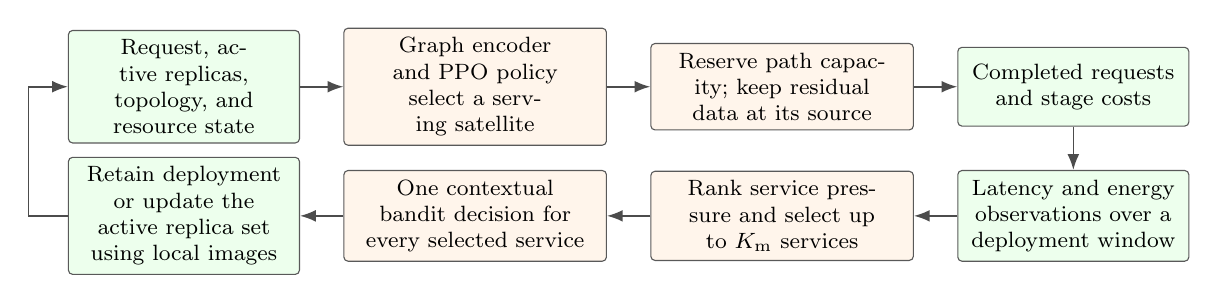
\begin{tikzpicture}[
    node distance=5.5mm and 5.5mm,
    box/.style={draw=black!65, rounded corners=1.5pt, align=center,
        minimum height=10mm, text width=29mm, fill=blue!4,
        font=\footnotesize},
    control/.style={box, fill=orange!8, text width=31mm},
    state/.style={box, fill=green!7, text width=27mm},
    flow/.style={-{Latex[length=2mm]}, line width=0.6pt, draw=black!70}
]
\node[state] (request) {Request, active replicas,\\topology, and resource state};
\node[control, right=of request] (select) {Graph encoder and PPO policy\\select a serving satellite};
\node[control, right=of select] (route) {Reserve path capacity; keep residual data at its source};
\node[state, right=of route] (outcome) {Completed requests\\and stage costs};

\node[state, below=of outcome] (summary) {Latency and energy observations over a deployment window};
\node[control, left=of summary] (pressure) {Rank service pressure and select up to $K_{\mathrm m}$ services};
\node[control, left=of pressure] (bandit) {One contextual bandit decision for every selected service};
\node[state, left=of bandit] (deployment) {Retain deployment or update the active replica set using local images};

\draw[flow] (request) -- (select);
\draw[flow] (select) -- (route);
\draw[flow] (route) -- (outcome);
\draw[flow] (outcome) -- (summary);
\draw[flow] (summary) -- (pressure);
\draw[flow] (pressure) -- (bandit);
\draw[flow] (bandit) -- (deployment);
\draw[flow] (deployment.west) -- ++(-5mm,0) |- (request.west);
\end{tikzpicture}
\caption{ELARA coordinates request execution and replica adaptation at two timescales. The fast control loop operates for each service stage. At a deployment window boundary, the slow control loop makes one decision for each of up to $K_{\mathrm m}$ services with the highest pressure.}
\label{fig:elara}
\vspace{-0.4cm}
\end{figure*}


\section{The Proposed ELARA Framework}
\label{sec:algo}
This section describes the two control loops used to implement the online decomposition in Sec.~\ref{sec:prob_form}. For each arriving request, the fast control loop selects a serving satellite for every microservice stage and routes its input data over the available ISLs. At deployment window boundaries, the slow control loop summarizes completed requests and updates replica placement. Both loops use the latency and energy cost in \eqref{eq:elara_prob_form}. Fig.~\ref{fig:elara} shows the resulting workflow.


\subsection{Serving Satellite Selection}

We formulate the sequential selection of serving satellites as a Markov decision process, where a complete episode corresponds to the execution of one request. To handle constellation topology that varies over time and heterogeneous computational resources, ELARA uses a PPO policy with a GNN to learn serving satellite selection.

\paragraph{State Space and GNN Representation}
For a given request $r = \langle v_{s}, m_{1}, \dots, m_{L}, v_{d}, \tau_{\text{in}} \rangle$, the $i$-th decision epoch is triggered when the required input data for microservice $m_{i}$ is ready on satellite $u_{r,i}$ at continuous time $\tau_{r,i}$. The system state is defined as a tuple:
\begin{equation}
s_{r,i} = (\mathcal{G}^{a}(t), u_{r,i}, v_{d}, \mathcal{M}_{r,i:L}, B_{r,i:L})
\end{equation}
where $t = s(\tau_{r,i})$ is the current decision slot, $\mathcal{M}_{r,i:L}$ and $B_{r,i:L}$ represent the sequence of pending service invocations and their corresponding data volumes, respectively. $\mathcal{G}^{a}(t)$ is an attributed SCPN graph defined as:
\begin{equation}
\mathcal{G}^{a}(t)=\big(\mathcal{V},\mathcal{E}(t),\mathcal{Q}^{v}(t),\mathcal{Q}^{e}(t)\big),
\end{equation}
where $\mathcal{Q}^{v}(t)$ denotes node states, including CPU capacity, computing queue length, service deployment, compute utilization, load state, and capacity discount factor.
Similarly, $\mathcal{Q}^{e}(t)$ captures link states, including ISL availability, effective transmission rate, link queue length, and propagation delay within the current time slot.

To enable the PPO agent to process the complex graph states, ELARA encodes each satellite $v$ with a feature vector $\mathbf{x}_{v}(t)$ for the current attributed graph $\mathcal{G}^{a}(t)$:
\begin{equation}
\begin{aligned}
\mathbf{x}_v(t)= [&\bar f_v,\bar q_v(t),\bar h_v(t),\bar p_v,\bar n_v,
\mathbb{I}_{v=u_{r,i}},\mathbb{I}_{v=v_d}, \\
&\mathbb{I}_{m_i\in v},\bar d_v(t),\mu_v(t),\xi_v(t),\ell_v(t)].
\end{aligned}
\end{equation}
%where the features capture normalized CPU frequency, compute queuing delay, hosted-service count, orbital-plane and intra-plane positions, source/destination indicators, current-service deployment, node degree, compute utilization, capacity discount, and load state.
where $\bar f_v$ is the CPU frequency, $\bar q_v(t)$ is the computation queueing delay, $\bar h_v(t)$ is the fraction of runtime memory occupied by active replicas, $\bar p_v$ is the orbital plane index, $\bar n_v$ is the relative position within that plane, $\mathbb{I}_{v=u_{r,i}}$ and $\mathbb{I}_{v=v_d}$ indicate whether $v$ is the current node and the destination node, respectively, $\mathbb{I}_{m_i\in v}$ indicates whether $m_i$ is active on $v$, $\bar d_v(t)$ is the node degree, $\mu_v(t)$ is the computation utilization, $\xi_v(t)$ is the computing capacity discount factor, and $\ell_v(t)$ is the computation load state.
The bar notation denotes a normalized value obtained using the corresponding numerical range.
%The request context is encoded as $\mathbf{c}_{r,i} = [\bar{L}_{r}, \bar{i}, \overline{L_{r}-i}, \bar{C}_{m_i}, \bar{B}_{r,i}, \bar{B}_{r}^{\text{rem}}]$, covering the chain length, stage index, remaining stages, CPU demand, current input size, and remaining data volume.
The request context is encoded as $\mathbf{c}_{r,i} = [\bar{L}_{r}, \bar{i}, \overline{L_{r}-i}, \bar{C}_{m_i}, \bar{B}_{r,i}, \bar{B}_{r}^{\text{rem}}]$, covering the chain length, $\bar{L}_{r}$, current stage index, $\bar{i}$, remaining stages, $\overline{L_{r}-i}$, required CPU cycles of $m_i$, $\bar{C}_{m_i}$, current input data volume, $\bar{B}_{r,i}$, and remaining data volume to be routed, $\bar{B}_{r}^{\text{rem}}$.
The request context is then projected into a latent embedding $\mathbf{z}_{r,i}=\sigma(\mathbf{W}_{c}\mathbf{c}_{r,i})$.

The GNN performs message passing over the active ISL graph to compute node embeddings.
Let $\mathbf{h}_v^{(0)}=\sigma(\mathbf{W}_0\mathbf{x}_v)$.
At GNN layer $l$, each satellite $v$ updates its representation by combining its current embedding with the mean embedding of its immediate neighbors:
\begin{equation}
\mathbf{h}_v^{(l+1)}
=\sigma\left(\mathbf{W}_{l}
\left[\mathbf{h}_v^{(l)},
\frac{1}{|\mathcal{N}_v|}\sum_{u\in\mathcal{N}_v}\mathbf{h}_u^{(l)}\right]\right).
\end{equation}
where $\mathcal{N}_{v}$ is the set of neighboring satellites of $v$, $\sigma(\cdot)$ is the activation function, and $\mathbf{W}_c$, $\mathbf{W}_0$, and $\mathbf{W}_{l}$ are trainable projection or transformation matrices.
The final embedding for node $v$ is denoted by $\mathbf{h}_{v}$.

\paragraph{Action Space}
Microservices may have different numbers of replicas, leading to action sets of different sizes for serving satellite selection.
For execution stage $i$, ELARA first ranks replicas by hop distance from $u_{r,i}$ and their current computing queue delay. It retains at most $N_{\text{cand}}$ replicas and removes nodes for which the routing procedure cannot find a feasible capacity reservation within the routing horizon. The resulting candidate set is
\begin{equation}
\mathcal{A}(s_{r,i})\subseteq\mathcal{R}_{m_i}(t),\qquad
|\mathcal A(s_{r,i})|\leq N_{\text{cand}}.
\end{equation}
Instead of using a fixed output layer over all satellites, ELARA applies a shared scorer to every node in $\mathcal A(s_{r,i})$ and normalizes the scores over this set.
\paragraph{Reward Function}
The reward is an additive decomposition of the request cost in \eqref{eq:request_cost_elara}. After stage $i$, ELARA assigns
\begin{align}
r_{r,i}=-\alpha\frac{T_{r,i}^{\text{step}}}{T_0}
-\beta\frac{E_{r,i}^{\text{step}}}{E_0},
\end{align}
where $T_{r,i}^{\text{step}}$ includes routing, queueing, and execution time, and $E_{r,i}^{\text{step}}$ includes communication and computation energy. The stage costs partition the measured request latency and energy, so their undiscounted reward sum equals $-J_r$ without repeated accounting. The PPO discount factor $\gamma$ controls temporal credit assignment during training.

\paragraph{PPO Policy and Update Mechanism}
%For each candidate $v \in \mathcal{A}(s_{r,i})$, ELARA constructs a 4-dimensional candidate feature vector $\mathbf{e}_{v}$, including normalized routing delay, transmission risk, bottleneck capacity shortage, and estimated computing cost.
%These features are derived from the routing and computing models in Sec.~\ref{sec:sys_model}.
%Specifically, the routing module estimates the delivery delay from $u_{r,i}$ to $v$, the future link unavailability risk, and the bottleneck capacity gap with respect to the required data volume.
%It also evaluates the outgoing capacity from $v$ to the next service stage or the destination, and uses the larger ingress or egress capacity shortage as the bottleneck feature.
%After the data arrival time is obtained, the onboard computing model estimates the queueing delay, execution delay, and computation energy on $v$, which together form the computing cost feature.
For each candidate $v \in \mathcal{A}(s_{r,i})$, ELARA constructs a feature vector $\mathbf{e}_{v}$ with four entries: the normalized routing delay from the current satellite $u_{r,i}$ to $v$, the risk of future link unavailability, the bottleneck ISL capacity gap, and the estimated computing cost at candidate node $v$. These features are computed using the routing and computing models described in Sec.~\ref{sec:sys_model}.
The policy network uses a multilayer perceptron (MLP) to score each candidate:
\begin{align}
g_\theta(v)=
\text{MLP}_{\theta}\big([\mathbf{h}_v,\mathbf{h}_{u_{r,i}},
\mathbf{h}_{v_d},\mathbf{z}_{r,i},\mathbf{e}_v]\big),
\end{align}
where $\mathbf{z}_{r,i}$ is the embedded request context vector.
A masked softmax is applied to ensure that action probabilities are distributed over legal candidates:
\begin{align}
\pi_{\theta}(v|s_{r,i}) = \frac{\exp(g_{\theta}(v))}{\sum_{v^{\prime}\in\mathcal{A}(s_{r,i})}\exp(g_{\theta}(v^{\prime}))}.
\end{align}

The value head $V_{\phi}(s_{r,i})$ estimates the expected return from the current state.
Using the generalized advantage estimate $\hat{A}_{j}$, ELARA updates the actor and critic networks by minimizing the following PPO loss function:
\begin{align}
\label{eq:ppo_loss}
\mathcal{L}(\theta,\phi)
=&-\mathbb{E}_{j}\!\left[\min(\rho_j\hat{A}_j,\bar{\rho}_j\hat{A}_j)\right] \nonumber\\
&+c_v\mathbb{E}_{j}\!\left[(V_{\phi}(s_j)-\hat{V}_j)^2\right]
-\eta_H\mathbb{E}_{j}\!\left[\mathcal{H}_j\right],
\end{align}
where $j$ is the index of a transition sampled from the PPO rollout buffer, $\rho_j=\pi_{\theta}(a_j|s_j)/\pi_{\theta_{\text{old}}}(a_j|s_j)$ is the original probability ratio, and $\bar{\rho}_j=\text{clip}(\rho_j,1-\epsilon,1+\epsilon)$ is the clipped ratio.
$\hat{V}_j$ is the value target and $\mathcal{H}_j=\mathcal{H}(\pi_{\theta}(\cdot|s_j))$ is the entropy term that encourages policy exploration.


\begin{algorithm}[t]
\SetAlFnt{\small}
\SetAlgoLined
\caption{Online Request Orchestration}
\label{algo:elara_request}
\SetKwInOut{Input}{Input}
\SetKwInOut{Output}{Output}
\Input{Request $r$, attributed graph snapshots $\{\mathcal{G}^{a}(t)\}$, trained policy $\pi_\theta$}
\Output{Serving nodes and routing paths}
$u\gets v_s$, $\tau\gets\tau_{\text{in}}$, $T_r\gets0$, $E_r\gets0$\;
\For{$i=1$ \KwTo $L$}{
Construct state $s_{r,i}$ and action space $\mathcal{A}(s_{r,i})$\;
Encode $\mathcal{G}^{a}(t)$ and request features by GNN\;
Select $v_{r,i}=\arg\max_v\pi_\theta(v|s_{r,i})$\;
Route $B_{r,i}$ from $u$ to $v_{r,i}$ using Algorithm~\ref{algo:cross_slot_routing}\;
Execute $m_i$ on $v_{r,i}$ and record $T_{r,i}^{\text{step}}$, $E_{r,i}^{\text{step}}$\;
$u\gets v_{r,i}$, $\tau\gets$ completion time of stage $i$\;
}
Route final output from $u$ to $v_d$ and compute $T_r^{\text{e2e}},E_r^{\text{tot}}$\;
\end{algorithm}
Algorithm~\ref{algo:elara_request} summarizes online inference. PPO training is performed offline using the reward and loss defined above.



\subsection{Data Routing across Time Slots}

For a selected pair $(u,v)$, ELARA attempts to deliver the stage input over at most $W_{\text{ru}}$ slots. In slot $t$, the controller constructs a residual graph from $\mathcal G(t)$. Let $A_e(t)$ denote the traffic already reserved on link $e$ during the remaining slot interval $\Delta_t$. The bit budget available to a new transmission is
\begin{equation}
C_e^{\text{res}}(t)=
\left[R_e(t)\left(\Delta_t-\nu_e^{\text{pr}}(t)
-\nu_e^{\text{qe}}(t)-\nu^{\text{sw}}\right)-A_e(t)\right]^+,
\label{eq:residual_capacity_routing}
\end{equation}
where $\nu^{\text{sw}}$ is the topology switching overhead. The reservation $A_e(t)$ contains active service traffic, so concurrent requests cannot reuse the same link capacity.

ELARA assigns each edge the cost
\begin{equation}
c_e(t)=\alpha\frac{\nu_e^{\text{qe}}(t)+\nu_e^{\text{pr}}(t)}{T_0}
+\beta\frac{P_e^{\text{tx}}}{E_0R_e(t)}+\chi\Gamma_e(t),
\label{eq:routing_edge_cost}
\end{equation}
where $\Gamma_e(t)$ indicates whether the link becomes unavailable within the routing horizon and $\chi$ controls the corresponding risk penalty. A successive shortest path procedure finds at most $K_{\text{max}}$ paths that do not share links. For each path, ELARA computes the largest data block that satisfies \eqref{eq:link_load_model} and can reach the selected satellite before the slot boundary. The capacity is reserved only after this condition is met.

Algorithm~\ref{algo:cross_slot_routing} gives the procedure. The key rule is that $B$ always denotes data still stored at $u$. A committed block is removed from $B$ only after the complete path has been admitted. If $B>0$ at the slot boundary, it remains at $u$ and the procedure starts from the updated topology in the next slot. Thus, topology changes do not create an unobserved buffer state at an intermediate satellite. The routing delay, energy, reserved capacity, and link risk are returned to the serving satellite selector as candidate features.

\begin{algorithm}[!t]
\SetAlFnt{\small}
\SetAlgoLined
\caption{Data Routing across Time Slots}
\label{algo:cross_slot_routing}
\SetKwInOut{Input}{Input}
\SetKwInOut{Output}{Output}
\Input{Source $u$, destination $v$, data size $B$, start time $\tau$}
\Output{Delivery time, energy, and link reservations}
\For{$h=1$ \KwTo $W_{\text{ru}}$}{
Construct the residual graph using \eqref{eq:residual_capacity_routing}\;
\For{$k=1$ \KwTo $K_{\max}$}{
Find the feasible path $p$ with minimum cost from $u$ to $v$\;
\If{no path exists}{break\;}
Compute the largest $d\leq B$ that can reach $v$ in the current slot\;
\If{$d=0$}{remove the bottleneck edge and continue\;}
Reserve $d$ bits on every edge of $p$ and set $B\gets B-d$\;
Remove the edges of $p$ from the request residual graph\;
\If{$B=0$}{\Return{delivery time, energy, and reservations}\;}
}
Keep $B$ at $u$ and set $\tau$ to the next slot boundary\;
}
\Return{no feasible reservation within the routing horizon}\;
\end{algorithm}


\subsection{Replica Adaptation}
The slow control loop considers replica updates every $Y_{\text{dep}}$ slots. Its design has three steps: rank the services, construct feasible actions, and learn whether retaining or changing a deployment reduces the common request cost. For an invocation of service $m$ at stage $i$ of request $r$, define
\begin{equation}
j_{r,i}=\alpha\frac{T_{r,i}^{\mathrm{ru}}+T_{r,i}^{\mathrm{cp}}}{T_0}
+\beta\frac{E_{r,i}^{\mathrm{ru}}+E_{r,i}^{\mathrm{cp}}}{E_0},
\label{eq:service_stage_cost}
\end{equation}
where $T_{r,i}^{\mathrm{cp}}$ includes the computation queueing delay in \eqref{eq:compute_delay_elara}. The normalized contribution of service $m$ in window $w$ is
\begin{equation}
I_{m,w}=
\frac{\sum_{(r,i)\in\mathcal I_{m,w}}j_{r,i}}
{\max\{\epsilon,\sum_{r\in\mathcal U_w}J_r\}},
\label{eq:service_impact}
\end{equation}
where $\mathcal I_{m,w}$ contains all completed invocations of $m$ in the window. A large contribution alone does not imply that relocation is useful. ELARA therefore measures adjustment potential from the tails of routing delay and computation queueing delay and from unequal use of the active replicas. Let $T_m^{\mathrm{ru}}(w)$ and $T_m^{\mathrm{qe}}(w)$ be the multisets of routing and queueing delay samples indexed by $\mathcal I_{m,w}$. Let $Q_q(\cdot)$ denote an empirical quantile, let $n_{m,v}$ be the number of invocations served by replica $v$, and let $\bar n_m$ be the mean over all active replicas of $m$. Then
\begin{equation}
\begin{aligned}
q_m^{\mathrm{ru}}=\left[\frac{Q_{0.95}(T_m^{\mathrm{ru}}(w))}
{\max\{\epsilon,Q_{0.50}(T_m^{\mathrm{ru}}(w))\}}-1\right]^+,\\
q_m^{\mathrm{qe}}=\left[\frac{Q_{0.95}(T_m^{\mathrm{qe}}(w))}
{\max\{\epsilon,Q_{0.50}(T_m^{\mathrm{qe}}(w))\}}-1\right]^+,
\end{aligned}
\label{eq:service_tail_pressure}
\end{equation}
and
\begin{equation}
q_m^{\mathrm{bal}}=
\left[\frac{\max_{v\in\mathcal R_m}n_{m,v}}
{\max\{\epsilon,\bar n_m\}}-1\right]^+.
\label{eq:service_balance_pressure}
\end{equation}
With $g(z)=z/(1+z)$, the raw pressure score is
\begin{equation}
\widetilde\psi_{m,w}=I_{m,w}\max\left\{g(q_m^{\mathrm{ru}}),
g(q_m^{\mathrm{qe}}),g(q_m^{\mathrm{bal}})\right\}.
\label{eq:service_pressure}
\end{equation}
An unavailable delay sample set contributes zero to the corresponding adjustment term. ELARA combines the current raw pressure with its preceding smoothed value using fixed exponential smoothing to reduce sensitivity to a single window. Before outcome samples are available, the invocation share initializes the ranking. ELARA selects up to $K_{\mathrm m}$ services with the largest smoothed pressure scores $\psi_{m,w}$. Every selected service receives one decision, but that decision may retain the current deployment.

For every selected service, ELARA identifies the source replica with the largest observed mean stage cost in \eqref{eq:service_stage_cost}. If its replicas have no stage cost observations, the least used replica is selected with deterministic tie breaking. For each other orbital plane, ELARA considers satellites that have enough free memory and do not already host an active replica of the same service. It retains the satellite with the smallest computation utilization in that plane, using memory utilization to break ties. The action set for service $m$ is
\begin{equation}
\mathcal A_{m,w}=\{\operatorname{retain}\}\cup
\{\operatorname{relocate}(v_m^-,v_{m,p}^+):p\in\mathcal P_{m,w}^{\mathrm{feas}}\},
\label{eq:replica_action_set}
\end{equation}
where $v_m^-$ is the source replica and $v_{m,p}^+$ is the selected satellite in plane $p$. ELARA processes the selected services in pressure order and updates the occupied memory after every relocation. Hence, every later action is constructed from the deployment produced by the preceding actions. At most one replica of each selected service is relocated, and the number of relocations in a window can range from zero to $K_{\mathrm m}$.

ELARA uses one shared linear contextual bandit for all services and actions. The context of action $a$ contains only the normalized service pressure, the expected communication cost from representative arrivals observed in the latest window, and the computation load at the satellite associated with the action:
\begin{equation}
\mathbf z_{m,a,w}=
\left[\widehat\psi_{m,w},\widehat C_{m,a,w}^{\mathrm{net}},
\widehat L_{a,w}^{\mathrm{cpu}}\right]^{\mathsf T}.
\label{eq:bandit_context}
\end{equation}
The pressure is normalized over the selected services, whereas network cost and computation load are normalized over $\mathcal A_{m,w}$. The expected communication cost uses the routing delay and energy terms with the same weights as \eqref{eq:request_cost_elara}. For the retention action, $v_m^-$ is used as the reference satellite for the two action dependent context entries. Let $\mathbf A$ and $\mathbf b$ be the shared model statistics and $\boldsymbol\theta=\mathbf A^{-1}\mathbf b$. The controller selects the action with the largest score
\begin{equation}
U(m,a,w)=\boldsymbol\theta^{\mathsf T}\mathbf z_{m,a,w}
+c\sqrt{\mathbf z_{m,a,w}^{\mathsf T}\mathbf A^{-1}\mathbf z_{m,a,w}},
\label{eq:contextual_ucb}
\end{equation}
where $c$ controls exploration. For $|\mathcal I_{m,w}|>0$, define the mean observed stage cost as $\bar j_{m,w}=|\mathcal I_{m,w}|^{-1}\sum_{(r,i)\in\mathcal I_{m,w}}j_{r,i}$. An action applied after window $w$ receives feedback after window $w+1$:
\begin{equation}
R_{m,w}=\frac{\bar j_{m,w}-\bar j_{m,w+1}}
{\max\{\epsilon,\bar j_{m,w}\}},
\label{eq:deployment_reward}
\end{equation}
where a missing observation in window $w+1$ produces zero feedback. The shared statistics are updated as $\mathbf A\leftarrow\mathbf A+\mathbf z\mathbf z^{\mathsf T}$ and $\mathbf b\leftarrow\mathbf b+R_{m,w}\mathbf z$. A retention action receives feedback in the same manner as a relocation, allowing the controller to learn when changing the deployment is unnecessary. An accepted relocation updates the active replica set using the local image at $v_{m,p}^+$. Because the pressure, context, and reward contain only observations associated with latency and energy, replica adaptation remains aligned with \eqref{eq:elara_prob_form}.



%The per-stage node selection complexity is $\mathcal{O}(L_g(|\mathcal{V}|+|\mathcal{E}|)d_h+|\mathcal{A}(s_{r,i})|d_h)$, where $L_g$ is the number of GNN layers and $d_h$ is the hidden dimension.
%For a look-ahead window of $W_{\text{ru}}$ time slots and at most $K_{\max}$ augmentations per time slot, the routing complexity is $\mathcal{O}(W_{\text{ru}}K_{\max}|\mathcal{E}|\log|\mathcal{V}|)$.
%For deployment, considering $K_s$ high-pressure services and $K_p$ target planes yields only $\mathcal{O}(K_sK_p|\mathcal{P}|)$ arms per round, avoiding exhaustive satellite-level service placement.

\section{Performance Evaluation}
\label{sec:eval}

%This section evaluates ELARA under dynamic LEO constellation topologies and microservice workloads.
%We aim to answer the following questions: (i) whether ELARA reduces end-to-end latency and energy compared with representative service orchestration baselines; (ii) whether its major components are all necessary; (iii) how the service-routing module behaves under different chain lengths; and (iv) whether adaptive replica redeployment provides sustained benefits over time.

\subsection{Experimental Setup}
We implement ELARA and all baselines in a discrete event simulator written in Python.
The simulator replays time varying LEO topology snapshots, maintains dynamic onboard computing queues and ISL queues, and records execution traces for requests and individual service stages.
Unless otherwise specified, each reported result is averaged over four random seeds.
\mbox{Table~\ref{tab:env_params}} summarizes the default constellation, workload, routing, and replica adaptation settings, whereas \mbox{Table~\ref{tab:learning_params}} lists the PPO, GNN, and bandit parameters. In particular, the default configuration uses 180 satellites, service chains of 5--15 microservices, a routing horizon of three slots, and an adaptation window of ten slots; these settings are kept fixed across the compared methods unless otherwise stated.

\begin{table}[!t]
\centering
\caption{Environment and Workload Parameters}
\label{tab:env_params}
\setlength{\tabcolsep}{2.8pt}
\scriptsize
\begin{tabular}{l|l}
\toprule
\textbf{Parameter} & \textbf{Default setting} \\
\midrule
Constellation size & 10 orbital planes, 18 satellites per plane \\
Time slot duration & 10 s \\
Time slots per cycle & 606 \\
Number of microservices & 30 \\
Replicas per microservice & 5--10 \\
Runtime memory per satellite & 12 GB \\
Runtime memory per microservice & 2.4--4.0 GB \\
Service image availability & Complete catalog on every satellite \\
CPU frequency & 1, 2, 3, or 4 GHz \\
Request chain length & 5, 10, or 15 \\
Request arrivals & Poisson process \\
Candidate replicas per stage $N_{\text{cand}}$ & 4 \\
Routing horizon $W_{\text{ru}}$ & 3 time slots \\
Maximum paths per time slot & 5 \\
Replica adaptation window & 10 time slots \\
\bottomrule
\end{tabular}
\vspace{-0.15cm}
\end{table}

\begin{table}[!t]
\centering
\caption{Learning Parameters}
\label{tab:learning_params}
\setlength{\tabcolsep}{2.8pt}
\scriptsize
\begin{tabular}{l|l}
\toprule
\textbf{Parameter} & \textbf{Default setting} \\
\midrule
GNN message passing layers & 2 \\
GNN/PPO hidden dimension & 128 \\
PPO learning rate & $3\times 10^{-4}$ \\
PPO discount factor & 0.99 \\
PPO clip parameter & 0.2 \\
PPO GAE parameter & 0.95 \\
PPO batch size & 64 \\
PPO rollout buffer size & 256 \\
Contextual UCB exploration factor $c$ & 1.25 \\
Services selected per window $K_{\mathrm m}$ & 8 \\
Bandit context dimension & 3 \\
\bottomrule
\end{tabular}
\vspace{-0.15cm}
\end{table}

The constellation contains 180 satellites and follows the slot based topology model in Sec.~\ref{sec:sys_model}.
Each microservice is associated with a CPU cycle demand and a runtime memory requirement. The memory settings permit approximately three to five active services on one satellite, depending on their individual requirements; the simulator does not impose a fixed service count per satellite.
All satellites store the same image catalog in persistent storage, so replica relocation uses local activation and deactivation without image traffic over ISLs.
Satellite CPUs are heterogeneous, and their effective computing capacities vary with background load states.
For communication, ISL capacities and propagation delays are obtained from the time varying topology snapshots, while queuing delay and effective rate degradation reflect background traffic.
Requests arrive according to a Poisson process and invoke sequential microservice chains.
The workload traces cover chain lengths of 5, 10, and 15, and are used consistently across the compared methods when request analyses are reported.

\begin{figure*}[!ht]
	\centering
	\begin{minipage}[!b]{0.42\textwidth}
		\centering
		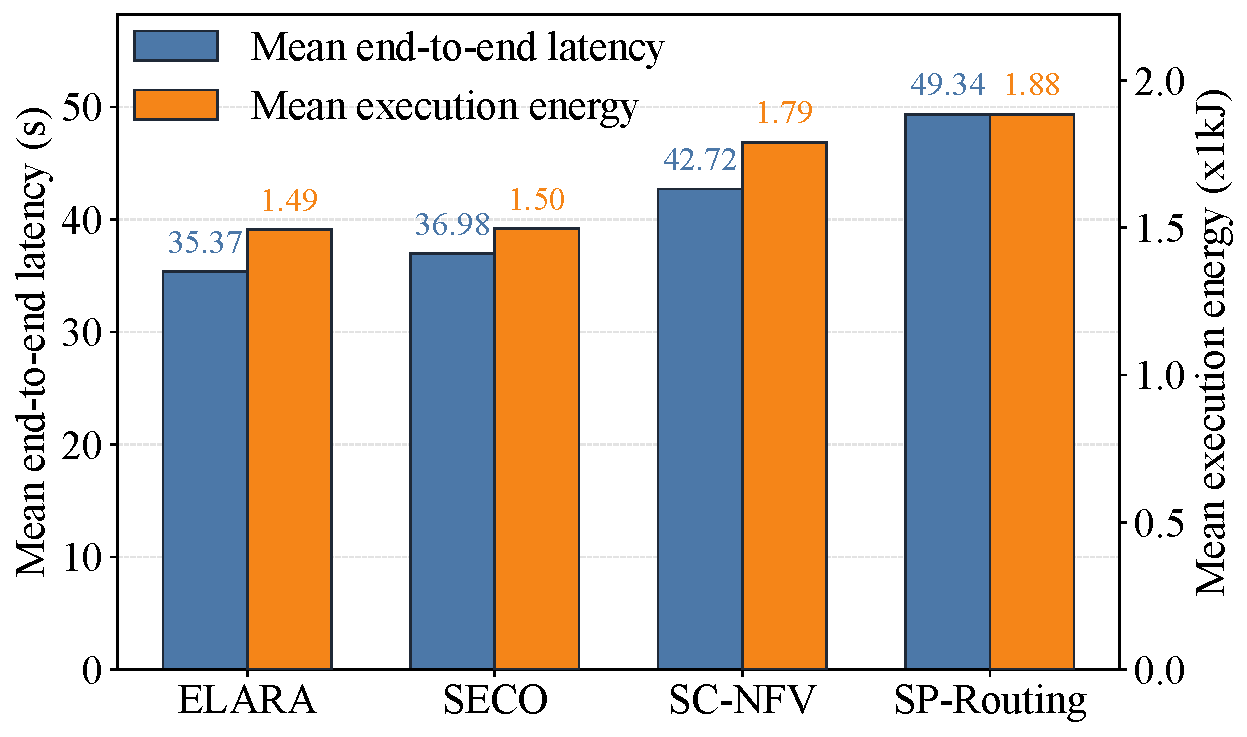
\includegraphics[width=1\linewidth]{elara_exp/elara_comparison.pdf}
		\vspace{-0.3cm}
		\caption{Performance against all baselines.}
		\label{fig:elara_comparison}
	\end{minipage}
	\hfill
	\begin{minipage}[!b]{0.42\textwidth}
		\centering
		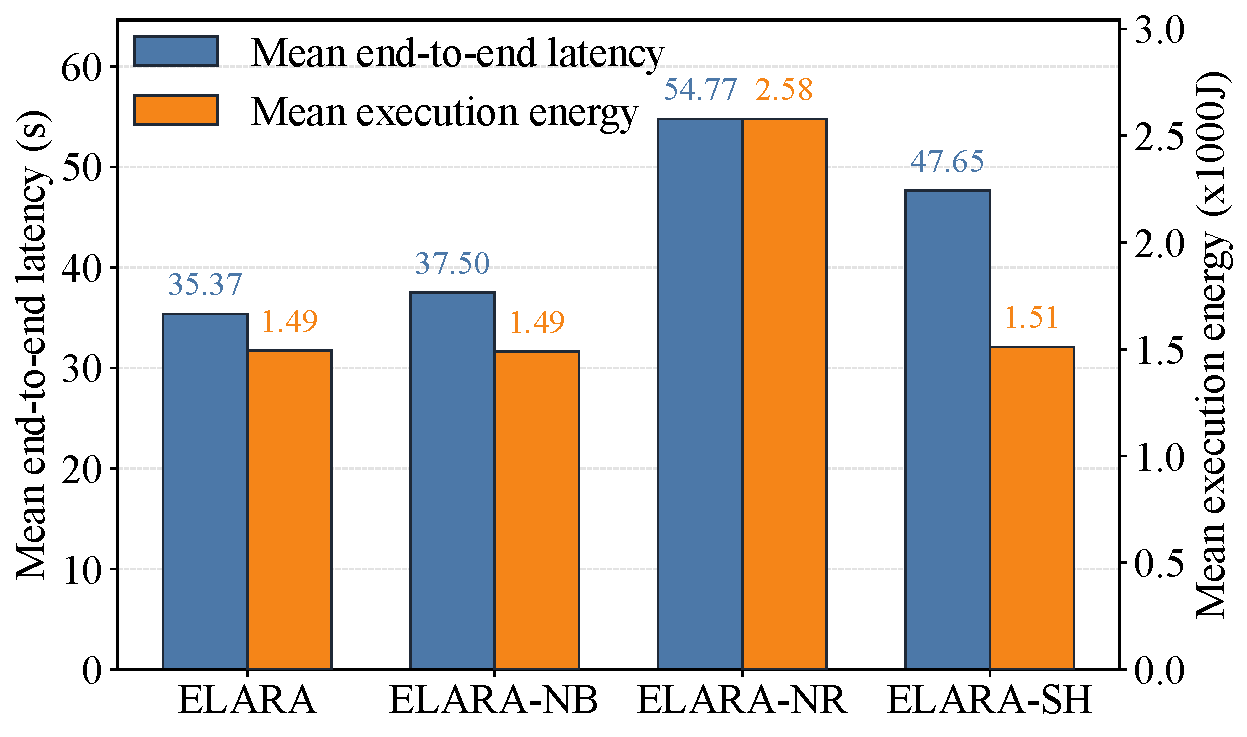
\includegraphics[width=1\linewidth]{elara_exp/elara_ablation.pdf}
		\vspace{-0.3cm}
		\caption{Ablation study of ELARA.}
		\label{fig:elara_ablation}
	\end{minipage}
	\vspace{-0.4cm}
\end{figure*}

\subsection{Baselines and Metrics}
We compare ELARA with the following baselines:
\begin{itemize}
\item \textbf{SECO}~\cite{seco_infocom2024}: a satellite edge computing baseline that performs processing and routing decisions according to queue states.
\item \textbf{SC-NFV}~\cite{sc_nfv_tmc2024}: a service chaining baseline adapted from satellite edge networks with network function virtualization to the considered microservice execution setting.
\item \textbf{SP-Routing}~\cite{service_pressure}: a service pressure routing baseline, inspired by backpressure, that favors nodes and paths with smaller virtual backlog.
\end{itemize}

For the ablation study, we further consider the following ELARA variants:
\begin{itemize}
\item \textbf{ELARA without adaptation}: disables the contextual bandit for replica adaptation.
\item \textbf{ELARA with nearest replica selection}: replaces the PPO policy with selection of the nearest replica.
\item \textbf{ELARA with shortest path routing}: replaces the proposed routing procedure across slots with shortest path routing.
\end{itemize}

We evaluate all methods using mean request latency, mean execution energy, mean communication delay, and the mean number of slot transitions.
Request latency includes both data routing and onboard computation, while execution energy includes communication and computation energy.
Slot transitions measure how often the transmission for a service stage spans multiple slots, thereby reflecting the ability of a method to handle dynamic ISL changes.

\subsection{Performance Evaluation}

\paragraph{Overall Performance.}
Fig.~\ref{fig:elara_comparison} compares ELARA with the representative baselines.
ELARA achieves the lowest average request latency of 35.37 s, reducing latency by 4.4\%, 17.2\%, and 28.3\% compared with SECO, SC-NFV, and SP-Routing, respectively.
The gains over SP-Routing and SC-NFV are larger because ELARA coordinates serving satellite selection with routing across slots and considers onboard computation states.
For mean execution energy, ELARA incurs 1.49 kJ, which is comparable to SECO and 16.6\% and 20.7\% lower than SC-NFV and SP-Routing, respectively.
These results show that optimizing routing pressure or service chain feasibility alone is insufficient, because serving satellite selection directly affects both communication and computation costs.

Fig.~\ref{fig:elara_ablation} studies the contribution of each ELARA component.
Removing replica adaptation increases the average latency from 35.37 s to 37.50 s, showing that placement updates can improve request execution as request patterns and topology states evolve.
Replacing the PPO node selector with nearest replica selection causes the largest degradation. This variant increases mean latency by 54.9\% and mean execution energy by 72.6\%, because it ignores onboard computation load, future routing risk, and ISL states, indicating that a satellite hosting a geographically nearby replica can be overloaded or poorly connected.
Replacing the proposed routing procedure with shortest path routing also degrades performance, increasing average latency by 34.7\%.
This result shows that hop count alone is a weak routing objective in dynamic LEO networks, where link availability, effective rate, queueing delay, and the amount left at the source for subsequent slots all affect routing performance.

\begin{figure}[!t]
\centering
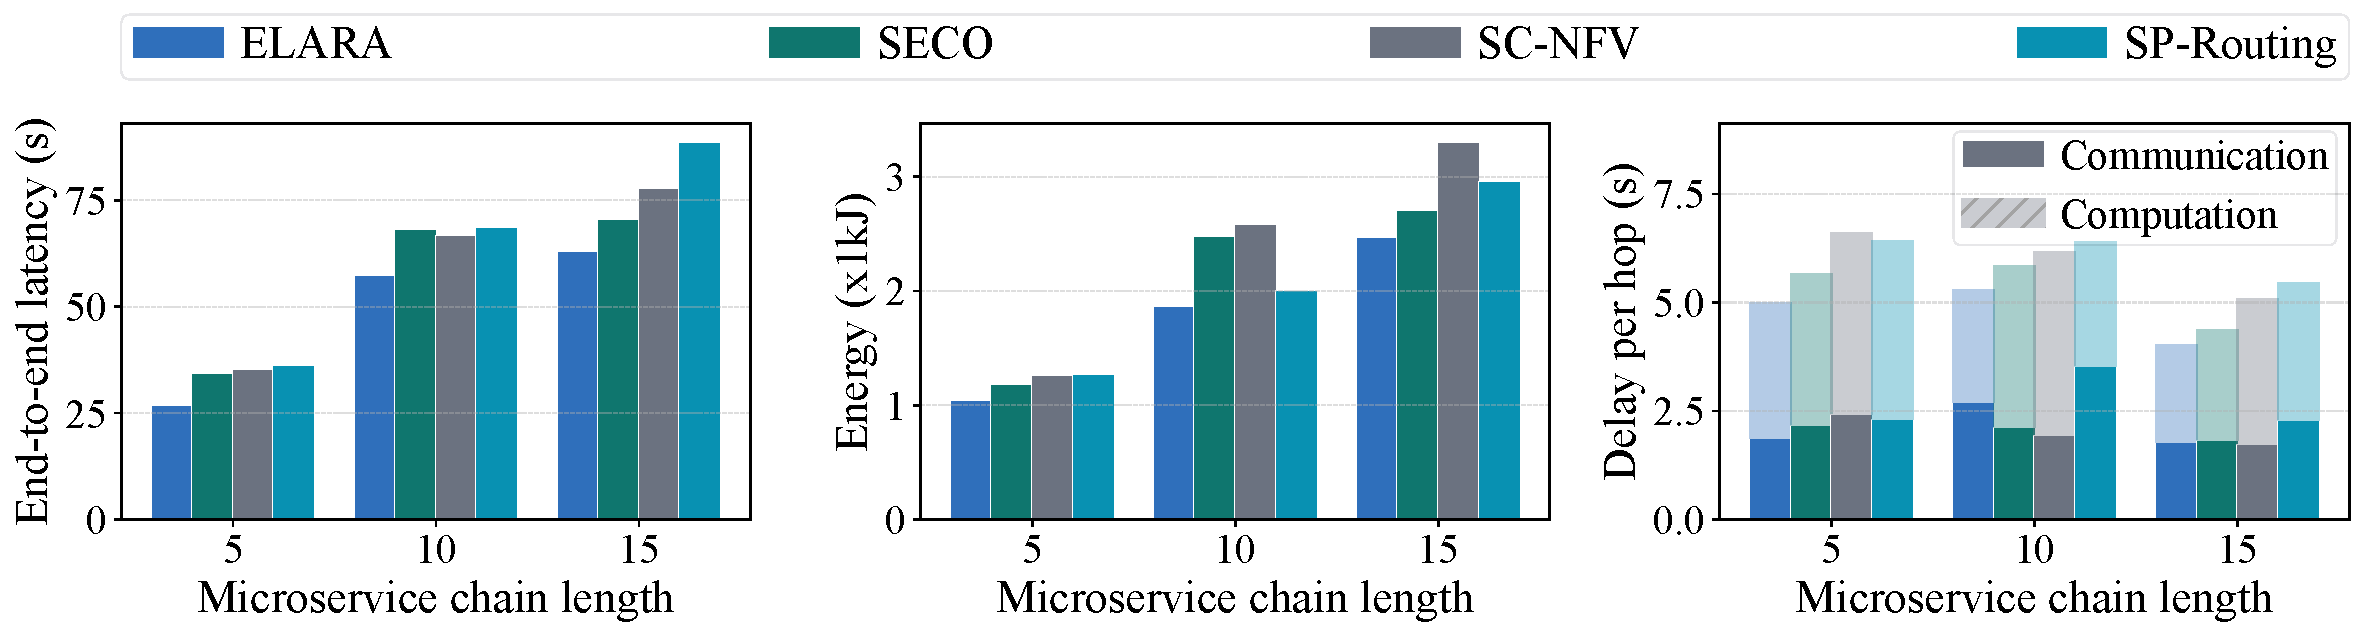
\includegraphics[width=1\linewidth]{elara_exp/service_routing_analysis_comparison.pdf}
\vspace{-0.6cm}
\caption{Service routing analysis against baselines.}
\label{fig:service_routing_analysis_comparison}
%	\vspace{-0.7cm}
\end{figure}

\begin{figure}[!t]
\centering
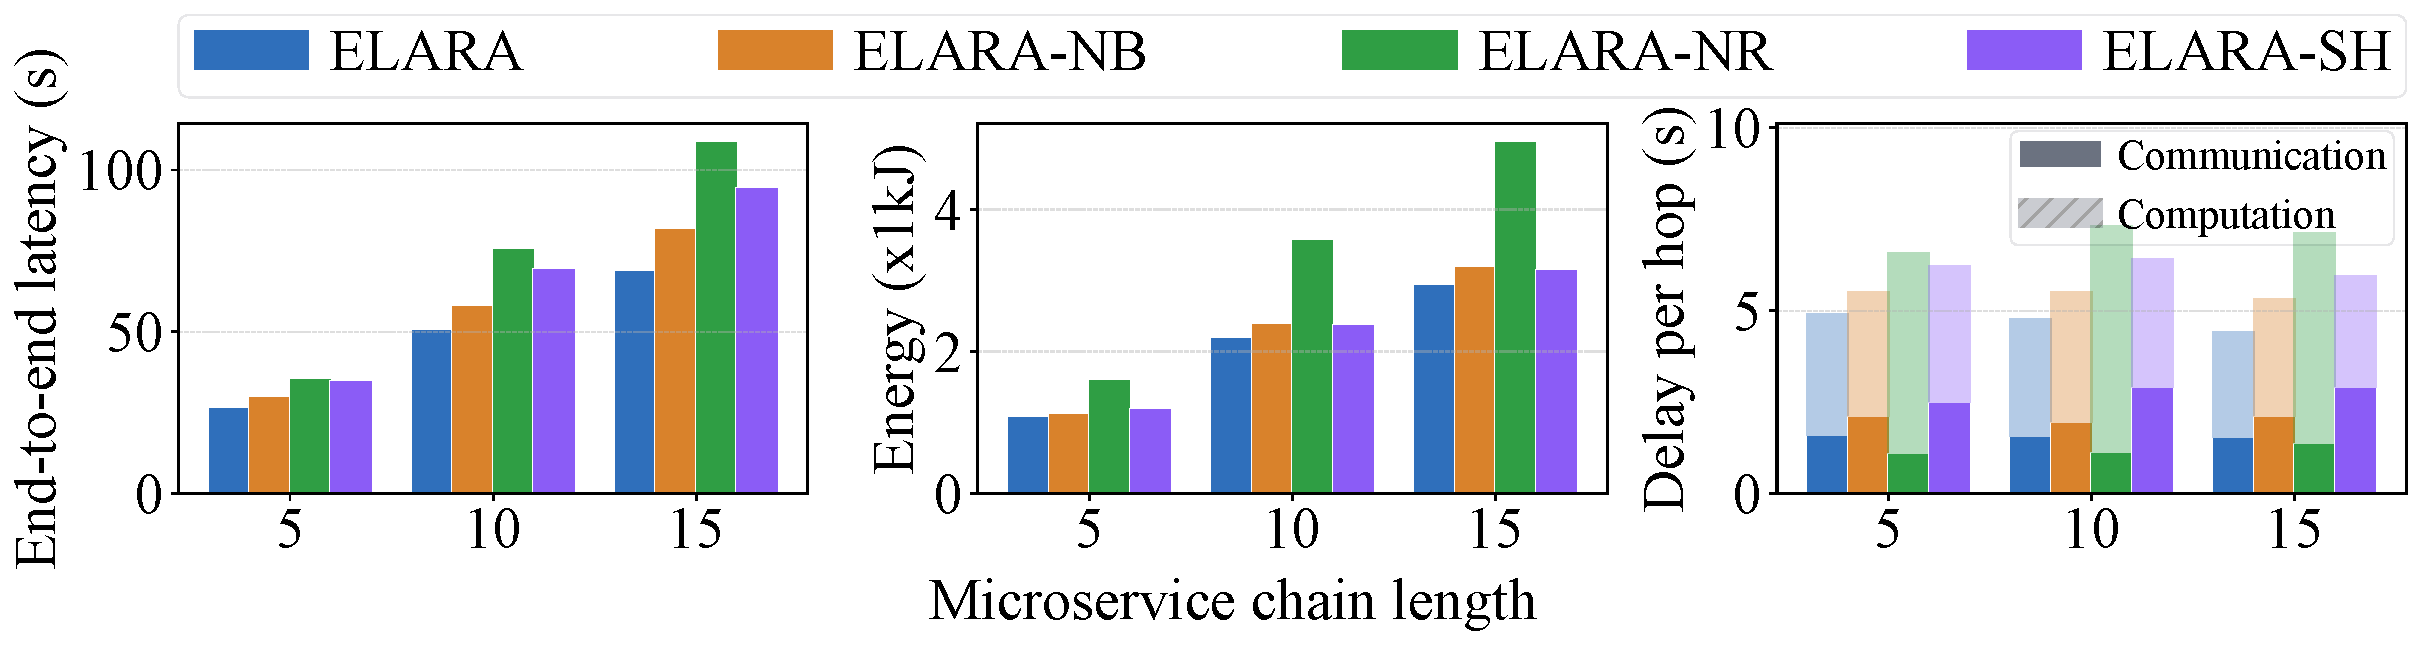
\includegraphics[width=1\linewidth]{elara_exp/service_routing_analysis.pdf}
\vspace{-0.6cm}
\caption{Service routing analysis against ELARA variants.}
\label{fig:service_routing_analysis}
\end{figure}

\paragraph{Service Routing Analysis}
Fig.~\ref{fig:service_routing_analysis_comparison} further examines requests and individual service stages under different chain lengths.
Across the analyzed traces, ELARA reduces request latency by about 15--24\% compared with SECO, SC-NFV, and SP-Routing.
Its mean execution energy is also consistently lower, with reductions of about 14--25\%.
The gain persists for longer service chains: for chain length 15, ELARA lowers the request latency by 10.6\% over SECO, 19.2\% over SC-NFV, and 29.0\% over SP-Routing.
These results show that ELARA's serving satellite selection is not only beneficial for isolated service stages, but also accumulates gains over a sequence of microservice executions.

Fig.~\ref{fig:service_routing_analysis} compares ELARA with its variants using common request traces.
ELARA reduces the average communication delay per hop by roughly 24\% over the variant without adaptation and 43\% over the variant with shortest path routing.
The shortest path variant suffers from larger communication delay because it may choose paths with fewer hops but insufficient effective rate or higher queuing delay.
In contrast, ELARA evaluates residual slot capacity and future link risk, allowing it to split traffic over multiple feasible paths when this lowers the overall delivery cost.
The nearest replica variant has shorter communication delay because it selects nearby replicas, but its much larger computation delay dominates the request latency.
This confirms that proximity alone is misleading when onboard computation heterogeneity and queuing states dominate service execution.

\section{Conclusion}
\label{sec:conclusion}
%In this paper, we proposed a DST-based solution to provide an energy-efficient service routing scheme for tasks from terrestrial clients. We systematically developed the SCPN models, including communication and computation, covering various aspects of the LEO satellite network. We also mathematically formulated the energy optimization problem for satellite-microservice routing and transformed it into finding a feasible DST solution within an augmented directed satellite-microservice colocated graph. To approximate the optimal solution, we designed a series of heuristic algorithms. Experimental results show that our algorithm significantly outperforms other benchmarks in energy efficiency, robustness, and adaptability across different network and microservice configurations in the context of SCPN.

This paper presented ELARA, an online microservice orchestration framework for dynamic SCPNs. Under one objective over the decision horizon, a fast control loop selects serving satellites and reserves ISL capacity along complete paths, while a slow control loop adapts replicas from request outcomes collected over each window. Undelivered data remains at the source and is routed again after each topology update. For up to $K_{\mathrm m}$ services with the highest pressure, a shared contextual bandit retains the current deployment or relocates one replica to another orbital plane subject to available memory. Relocation updates the active replica set using images stored locally on each satellite. Simulations with dynamic LEO traces show that coordinating request execution, routing, and replica adaptation reduces latency and energy compared with representative baselines.



% if have a single appendix:
%\appendix[Proof of the Zonklar Equations]
% or
%\appendix  % for no appendix heading
% do not use \section anymore after \appendix, only \section*
% is possibly needed

% use appendices with more than one appendix
% then use \section to start each appendix
% you must declare a \section before using any
% \subsection or using \label (\appendices by itself
% starts a section numbered zero.)
%


% \appendices
% \section{Proof of the First Zonklar Equation}
% Appendix one text goes here.

% % you can choose not to have a title for an appendix
% % if you want by leaving the argument blank
% \section{}
% Appendix two text goes here.


% use section* for acknowledgment
% \section*{Acknowledgment}



% Can use something like this to put references on a page
% by themselves when using endfloat and the captionsoff option.
\ifCLASSOPTIONcaptionsoff
\newpage
\fi



% trigger a \newpage just before the given reference
% number - used to balance the columns on the last page
% adjust value as needed - may need to be readjusted if
% the document is modified later
%\IEEEtriggeratref{8}
% The "triggered" command can be changed if desired:
%\IEEEtriggercmd{\enlargethispage{-5in}}

% references section

\bibliographystyle{ieeetr}
\bibliography{ref.bib}

% biography section
%
% If you have an EPS/PDF photo (graphicx package needed) extra braces are
% needed around the contents of the optional argument to biography to prevent
% the LaTeX parser from getting confused when it sees the complicated
% \includegraphics command within an optional argument. (You could create
% your own custom macro containing the \includegraphics command to make things
% simpler here.)
%\begin{IEEEbiography}[{\includegraphics[width=1in,height=1.25in,clip,keepaspectratio]{mshell}}]{Michael Shell}
% or if you just want to reserve a space for a photo:

% \begin{IEEEbiography}{Michael Shell}
% Biography text here.
% \end{IEEEbiography}

% if you will not have a photo at all:
% \begin{IEEEbiographynophoto}{John Doe}
% Biography text here.
% \end{IEEEbiographynophoto}

% insert where needed to balance the two columns on the last page with
% biographies
%\newpage

% \begin{IEEEbiographynophoto}{Jane Doe}
% Biography text here.
% \end{IEEEbiographynophoto}

% You can push biographies down or up by placing
% a \vfill before or after them. The appropriate
% use of \vfill depends on what kind of text is
% on the last page and whether or not the columns
% are being equalized.

%\vfill

% Can be used to pull up biographies so that the bottom of the last one
% is flush with the other column.
%\enlargethispage{-5in}



% that's all folks
\end{document}
